\documentclass[border=10pt]{standalone}
\usepackage[svgnames]{xcolor}
\usepackage{amsmath}
\usepackage{pgfplots}
\pgfplotsset{compat=newest}
\usepackage[sfdefault]{FiraSans}
\usepackage{FiraMono}
\renewcommand*\familydefault{\sfdefault}
\begin{document}
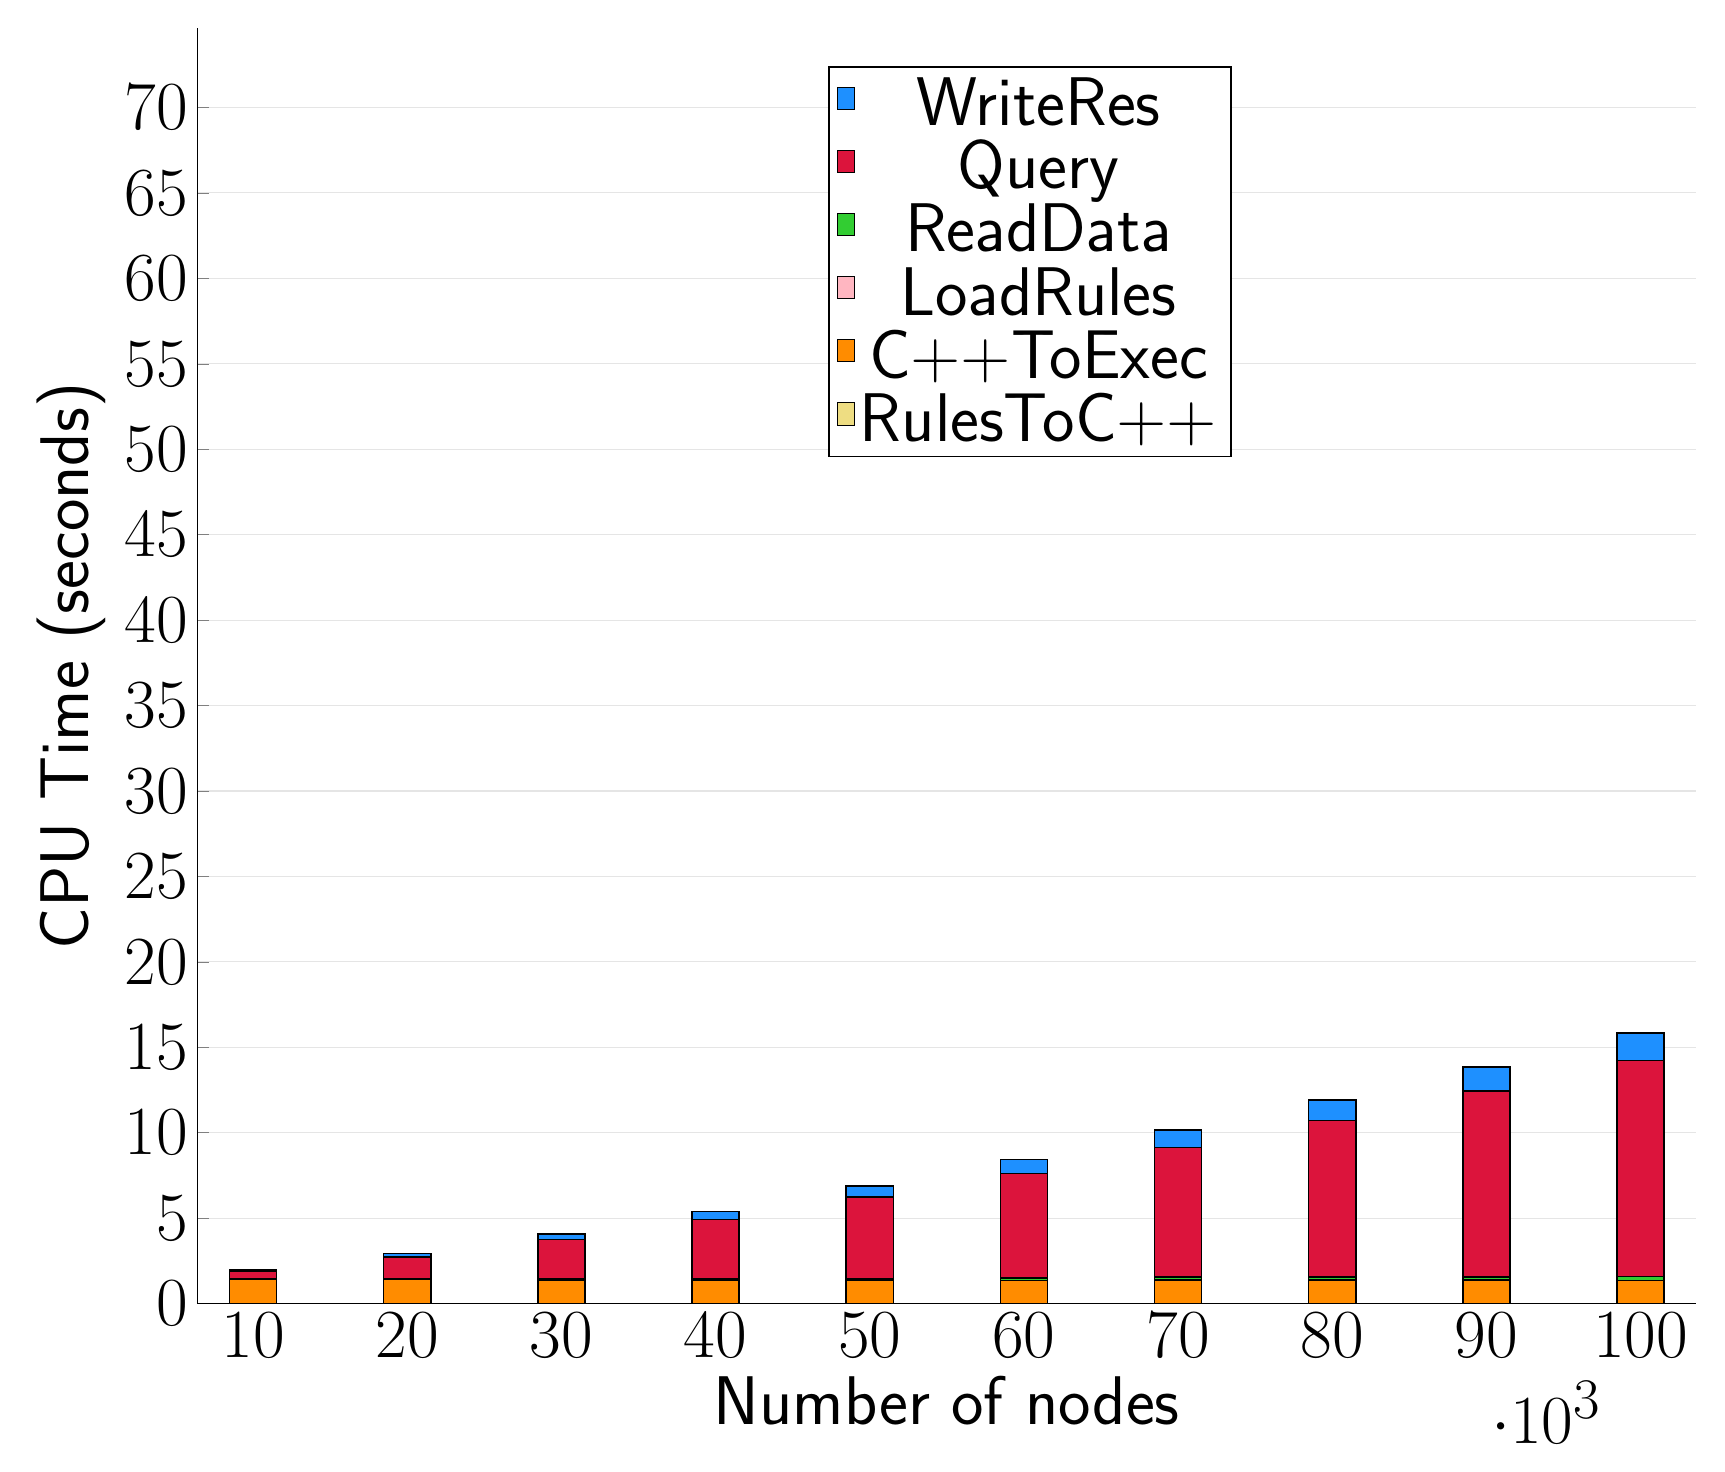
\begin{tikzpicture}
\begin{axis}[
   ybar stacked,
   width=1.7\textwidth,
   bar width=0.6cm,
   ymajorgrids, tick align=inside,
   major grid style={draw=gray!20},
   xtick=data,
   scaled x ticks={base 10:-3},
   ymin=0, ymax=74.64057999999999,
   axis x line*=bottom,
   axis y line*=left,
   enlarge x limits=0.04,
   legend style={
       at={(0.69, 0.97)},
       anchor=north east,
       legend columns=1,
       font=\Huge,
   },
   ylabel={CPU Time (seconds)},
   xlabel={Number of nodes},
   label style={font=\Huge},
   tick label style={font=\Huge},
]
\addlegendimage{fill=DodgerBlue, draw=black, line width=0.2pt}
\addlegendentry{WriteRes}
\addlegendimage{fill=Crimson, draw=black, line width=0.2pt}
\addlegendentry{Query}
\addlegendimage{fill=LimeGreen, draw=black, line width=0.2pt}
\addlegendentry{ReadData}
\addlegendimage{fill=LightPink, draw=black, line width=0.2pt}
\addlegendentry{LoadRules}
\addlegendimage{fill=DarkOrange, draw=black, line width=0.2pt}
\addlegendentry{C++ToExec}
\addlegendimage{fill=LightGoldenrod, draw=black, line width=0.2pt}
\addlegendentry{RulesToC++}
\addplot +[fill=LightGoldenrod, draw=black, line width=0.55pt] coordinates {
(10000, 0.0020000000000000018)
(20000, 0.004000000000000001)
(30000, 0.0020000000000000018)
(40000, 0.0)
(50000, 0.0)
(60000, 0.0)
(70000, 0.0020000000000000018)
(80000, 0.0)
(90000, 0.0)
(100000, 0.0)
};
\addplot +[fill=DarkOrange, draw=black, line width=0.55pt] coordinates {
(10000, 1.4000000000000001)
(20000, 1.3980000000000004)
(30000, 1.374)
(40000, 1.3800000000000001)
(50000, 1.3679999999999999)
(60000, 1.352)
(70000, 1.3920000000000001)
(80000, 1.3719999999999999)
(90000, 1.3719999999999999)
(100000, 1.3640000000000003)
};
\addplot +[fill=LightPink, draw=black, line width=0.55pt] coordinates {
(10000, 0.00011819999999999999)
(20000, 0.0001594)
(30000, 0.00015639999999999998)
(40000, 0.0001698)
(50000, 0.0001496)
(60000, 0.0001546)
(70000, 0.00015580000000000002)
(80000, 0.0001496)
(90000, 0.0001588)
(100000, 0.0001374)
};
\addplot +[fill=LimeGreen, draw=black, line width=0.55pt] coordinates {
(10000, 0.029142399999999995)
(20000, 0.0557594)
(30000, 0.0765446)
(40000, 0.0956922)
(50000, 0.1141262)
(60000, 0.1355834)
(70000, 0.15330819999999998)
(80000, 0.1738858)
(90000, 0.1927336)
(100000, 0.21162959999999997)
};
\addplot +[fill=Crimson, draw=black, line width=0.55pt] coordinates {
(10000, 0.4762168)
(20000, 1.2828579999999998)
(30000, 2.2877520000000002)
(40000, 3.4511600000000002)
(50000, 4.759838)
(60000, 6.118422)
(70000, 7.59461)
(80000, 9.167995999999999)
(90000, 10.886940000000001)
(100000, 12.6399)
};
\addplot +[fill=DodgerBlue, draw=black, line width=0.55pt] coordinates {
(10000, 0.0744394)
(20000, 0.1899006)
(30000, 0.3271646)
(40000, 0.47634920000000003)
(50000, 0.6434504000000001)
(60000, 0.8145236)
(70000, 1.010414)
(80000, 1.198488)
(90000, 1.4093740000000001)
(100000, 1.6152460000000002)
};
\end{axis}
\end{tikzpicture}

\end{document}
